\documentclass[10pt,a4paper,twoside,onecolumn]{article}
\usepackage[utf8]{inputenc}
\usepackage[bitstream-charter]{mathdesign}
\usepackage{amsmath}
\usepackage{graphicx}
\usepackage{multicol}
\usepackage{xcolor}
\usepackage{titlesec}
\usepackage[sfdefault,condensed]{roboto}
\usepackage[left=2cm, right=2cm]{geometry}
\usepackage{fancyhdr}
\fancyhead[CE]{}
\fancyhead[LE]{REPORTS}
\fancyhead[RE]{\rightmark}
\fancyhead[CO]{}
\fancyhead[LO]{\leftmark}
\fancyhead[RO]{REPORTS}
\fancyfoot[CE]{4 FEBRUARY 2011 VOL 331 \textbf{SCIENCE} www.sciencemag.org}
\fancyfoot[LE]{\thepage}
\fancyfoot[RE]{}
\fancyfoot[CO]{4 FEBRUARY 2011 VOL 331 \textbf{SCIENCE} www.sciencemag.org}
\fancyfoot[LO]{}
\fancyfoot[RO]{\thepage}
\pagestyle{fancy}
\usepackage{graphicx}
%Note verticale
\usepackage[all]{background}
\usepackage{url}
\usepackage{hyperref}
\usepackage{color}
\SetBgContents{\textcolor{black}{Downloaded from \url{ www.sciencemag.org} on February 3, 2011}}% Set contents
\SetBgPosition{18cm,-10cm}% Select location
\SetBgOpacity{1.0}% Select opacity
\SetBgAngle{90.0}% Select rotation of logo
\SetBgScale{1.0}% Select scale factor of logo


\newcommand*{\myfont}{\fontfamily{<pbk>}\selectfont}

\author{Liz}
\begin{document}
\setcounter{page}{578}
{\Huge\textbf{2500 Years of European Climate Variability and Human Susceptibility }}
%\author[1]{y} check author affiliations authblk pkg
%\affil[1]{x}

{\small Ulf Büntgen,$^{1,2,\ast}$ Willy Tegel,$^{3}$ Kurt Nicolussi,$^{4}$ Michael McCormick,$^{5}$ David Frank,$^{1,2}$ Valerie Trouet,$^{1,6}$,
Jed O. Kaplan,$^{7}$ Franz Herzig,$^{8}$ Karl-Uwe Heussner,$^{9}$ Heinz Wanner,$^{2}$ Jürg Luterbacher,$^{10}$ Jan Esper$^{11}$} \footnote{$^{1}$Swiss Federal Research Institute for Forest, Snow and Landscape Research (WSL), 8903 Birmensdorf, Switzerland.
$^{2}$Oeschger Centre for Climate Change Research, University of Bern, 3012 Bern, Switzerland.
$^{3}$Institute for Forest Growth,University of Freiburg, 79085 Freiburg, Germany.
$^{4}$Institute of Geography, University of Innsbruck, 6020 Innsbruck, Austria.
$^{5}$Department of History,
Harvard University, Cambridge, MA 02138, USA.
$^{6}$Laboratory of Tree-Ring Research, University of Arizona, Tucson, AZ 85721, USA.
$^{7}$Environmental Engineering Institute, École Polytechnique
Fédérale de Lausanne, 1015 Lausanne, Switzerland.
$^{8}$Bavarian State Department for Cultural Heritage, 86672 Thierhaupten,
Germany.
$^{9}$German Archaeological Institute, 14195 Berlin, Germany.
$^{10}$Department of Geography, Justus Liebig University, 35390 Giessen,
Germany.
$^{11}$Department of Geography, Johannes Gutenberg University,
55128 Mainz, Germany.
$^{\ast}$To whom correspondence should be addressed. E-mail: buentgen@wsl.ch}


\textbf{Climate variations influenced the agricultural productivity, health risk, and conflict level of preindustrial societies. Discrimination between environmental and anthropogenic impacts on past civilizations, however, remains difficult because of the paucity of high-resolution paleoclimatic evidence. We present tree ring–based reconstructions of central European summer precipitation
and temperature variability over the past 2500 years. Recent warming is unprecedented, but modern hydroclimatic variations may have at times been exceeded in magnitude and duration. Wet and warm summers occurred during periods of Roman and medieval prosperity. Increased climate variability from ~250 to 600 C.E. coincided with the demise of the western Roman Empire and the turmoil of the Migration Period. Such historical data may provide a basis for counteracting the recent political and fiscal reluctance to mitigate projected climate change.}
\begin{myfont}
	\begin{multicols}{3}
{\huge C}ontinuing global warming and its potential associated threats to ecosystems and human health present a substantial challenge
to modern civilizations that already experience many direct and indirect impacts of anthropogenic climate change (1–4). The rise and fall of
past civilizations have been associated with environmental change, mainly due to effects on water supply and agricultural productivity (5–9), human
health (10), and civil conflict (11). Although many lines of evidence now point to climate forcing as one agent of distinct episodes of societal
crisis, linking environmental variability to human history is still limited by the dearth of high resolution paleoclimatic data for periods earlier than
1000 years ago (12). \par
Archaeologists have developed oak (\textit{Quercus spp.}) ring width chronologies from central Europe that cover nearly the entire Holocene and have used them for the purpose of dating archaeological artifacts, historical buildings, antique artwork, and furniture (13). The number of samples contributing to these records fluctuates between hundreds and thousands in periods of societal prosperity, whereas fewer samples from periods of socioeconomic instability are available (14). Chronologies of living (15) and relict oaks (16, 17) may reflect distinct patterns of summer precipitation and drought if site ecology and local climatology imply moisture deficits during the vegetation period. Annually resolved climate reconstructions that contain long-term trends and extend prior to
medieval times, however, depend not only on the inclusion of numerous ancient tree-ring samples of sufficient climate sensitivity, but also on frequency
preservation, proxy calibration, and uncertainty estimation (18–20). \par
To better understand interannual to multicentennial changes in central European April-to-June (AMJ) precipitation over the late Holocene, we used 7284 precipitation-sensitive oak ringwidth series from subfossil, archaeological, historical, and recent material representing temperate forests
in northeastern France (NEF), northeastern Germany (NEG), and southeastern Germany (SEG) (Fig. \ref{Fig1}). We found that themean annual replication was 286
series,with a maximum of 550 series during Roman times and the smallest sample size of 44 series at ~400 C.E. Growth variations among the three
regions were significantly (P < 0.001) correlated over the past two millennia: NEF/SEG at 0.53, SEG/NEG at 0.47, and NEF/NEG at 0.37 (21). Correlation coefficients among AMJ precipitation readings fromthree stations in NEF, NEG, and SEG averaged 0.31 over the common instrumental period (1921 to 1988), whereas the three regional oak chronologies correlated at 0.37 over the same interval (21). \par
	\end{multicols}	
\begin{figure}[h] %on ouvre l'environnement figure
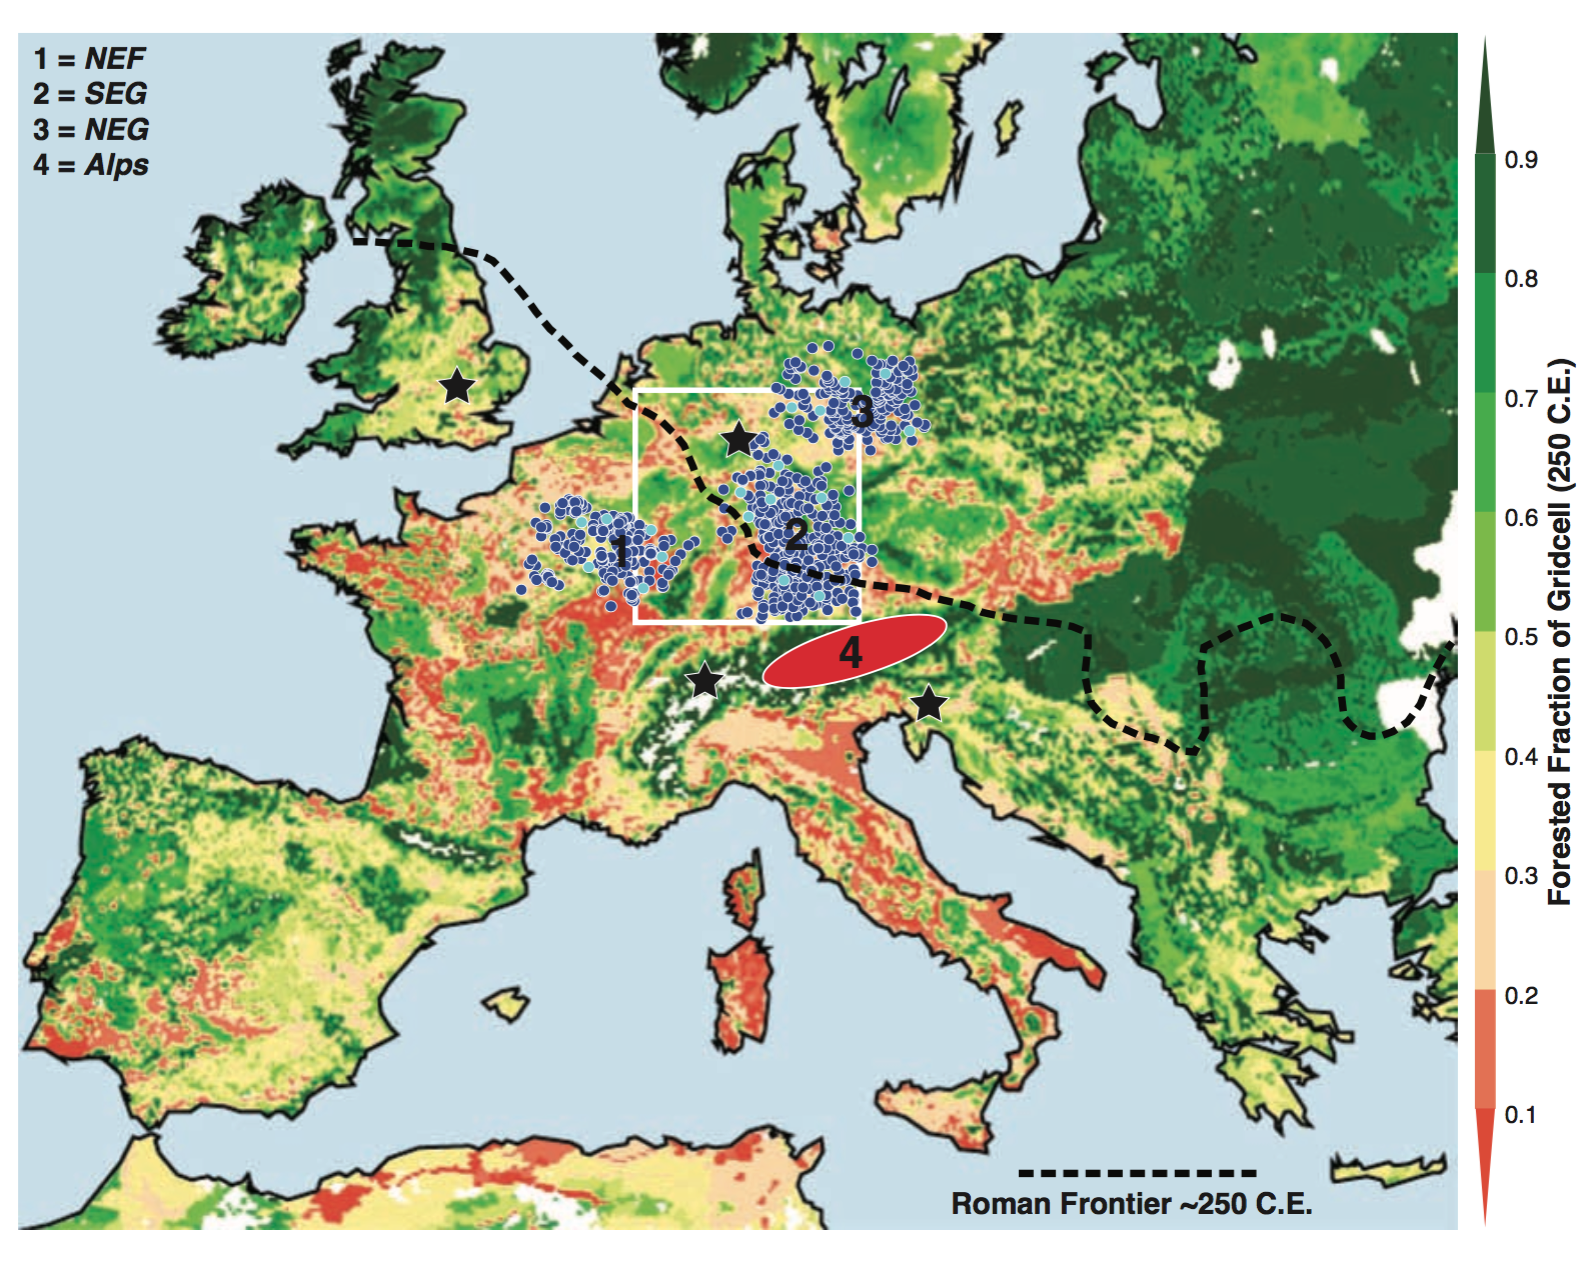
\includegraphics[width=1\textwidth]{BuntgenFig1}
\caption{Location of the 7284 central European oak samples (blue) and the net- work of 1546 Alpine coni- fers (red), superimposed on a deforestation model of Roman land use and land cover around 250 C.E. (22). Black stars indicate the lo- cation of the independent tree-ring chronologies used for comparison (16–19); the white box denotes the area over which gridded precipita- tion totals were averaged and used for proxy calibration.} %la légende
\label{Fig1} %l'étiquette pour faire référence à cette image
\end{figure} %on ferme l'environnement figure
	\begin{multicols}{3}
The temporal distribution of historical tree harvest (i.e., felling dates) mimics preindustrial deforestation and population trends (Fig. \ref{Fig2}),
implying substantial anthropogenic landscape perturbation over the last 2500 years (22). Increased felling dates reflect construction activity
during the late Iron Age and Roman Empire (~300 B.C.E. to 200 C.E.) and indicate that the maximum expansion and deforestation of the
Western Roman Empire (WRE) occurred around 250 C.E. Reduced tree harvesting at ~250 to 400 C.E. coincides with the biggest central European
historical crisis, the Migration Period, a time marked by lasting political turmoil, cultural change, and socioeconomic instability (23, 24).
Increasing timber harvest for construction is represented by abundant felling parallel to socioeconomic consolidation from the 6th to the 9th
centuries C.E. Many earlier structures were replaced during a settlement boom in the 13th century (23, 24), eliminating much construction
evidence from the central medieval period (900 to 1100 C.E.). Construction activity during the last millennium was disrupted by the Great Famine
and Black Death (19) as well as by the Thirty Years’ War. \par
	\end{multicols}	
\begin{figure}[h]
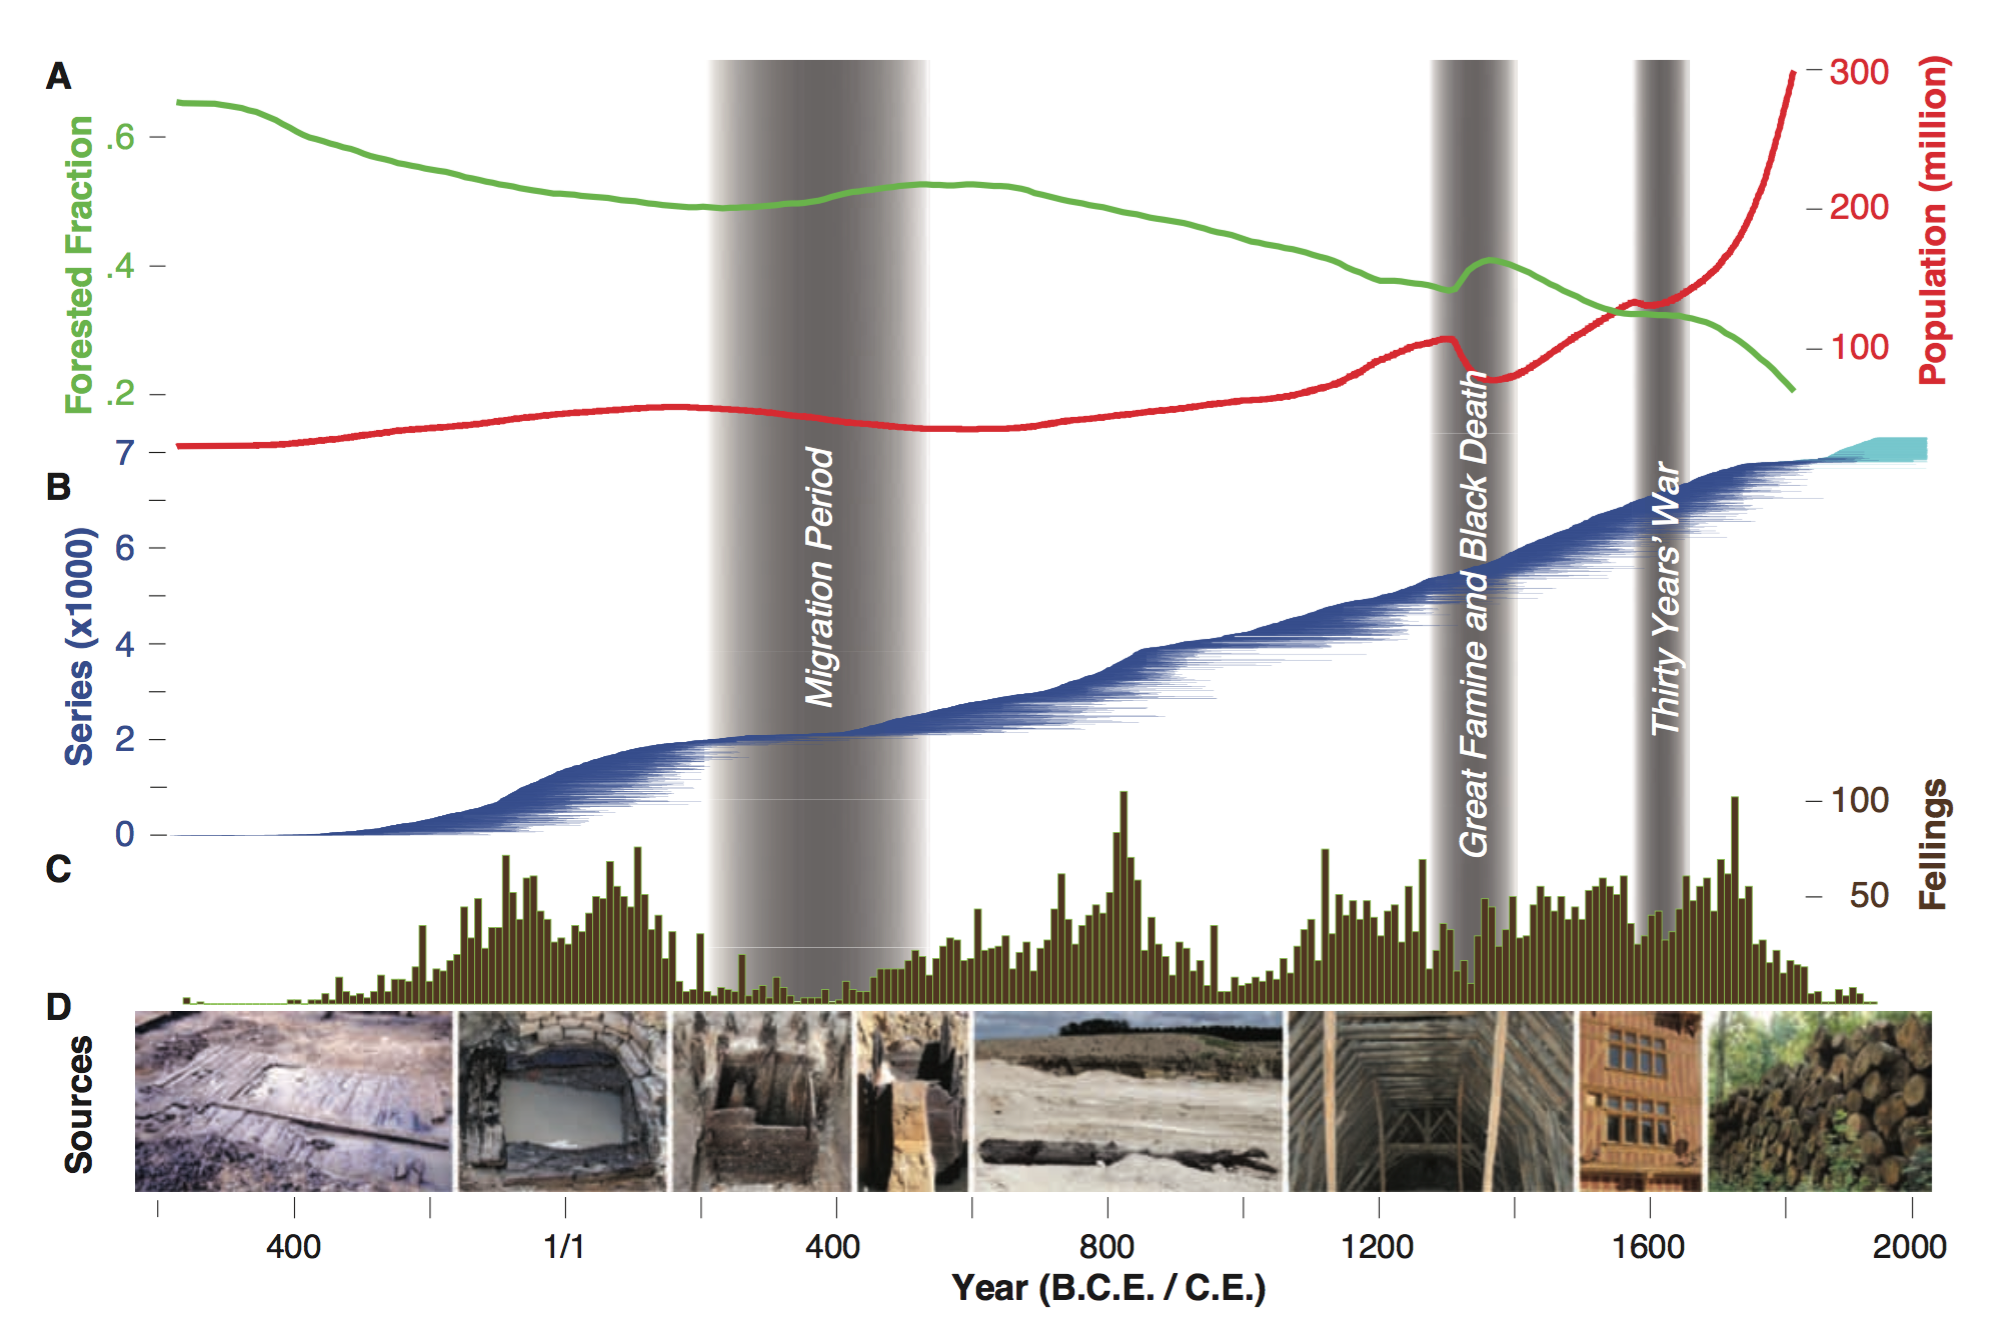
\includegraphics[width=1\textwidth]{BuntgenFig2}
\caption{(\textbf{A} to \textbf{D}) Evolution of central European forest cover and population from ( 22) (A), together with oak sample replication (B), their historical end dates at decadal resolution (C), and examples of archaeological (left), subfossil, historical, and recent (right) sample sources (D).} 
\label{Fig2} 
\end{figure}
	\begin{multicols}{3}
To assess climatic drivers of oak growth during industrial and preindustrial times, we compared chronologies of high-frequency variability
with instrumental records, independent climate reconstructions, and historical archives (21). A total of 87 different medieval written sources
comprise 88 eyewitness accounts of regional hydroclimatic conditions (with as many as seven reports per year) resolved to the year or better,
which corroborate 30 out of 32 of the extremes preserved in our oak record between 1013 and 1504 C.E., whereas 16 reports were found to be
contradictory (Fig. \ref{Fig3}A). These observations further confirm the spatial signature of the climatic signal reflected by the oak network. Scaled precipitation
anomaly composites calculated for the 12 most positive and the 16 most negative oak extremes back to 1500 C.E. revealed significantly
wet and dry central European summers, respectively (Fig. \ref{Fig3}B) (21). Independently derived extremes in pan-European oak growth over the
last millennium match 5 of 11 extremes at the central European network level, and 21 of 53 at the regional scale (fig. S6). \par
	\end{multicols}	
\begin{figure}[h]
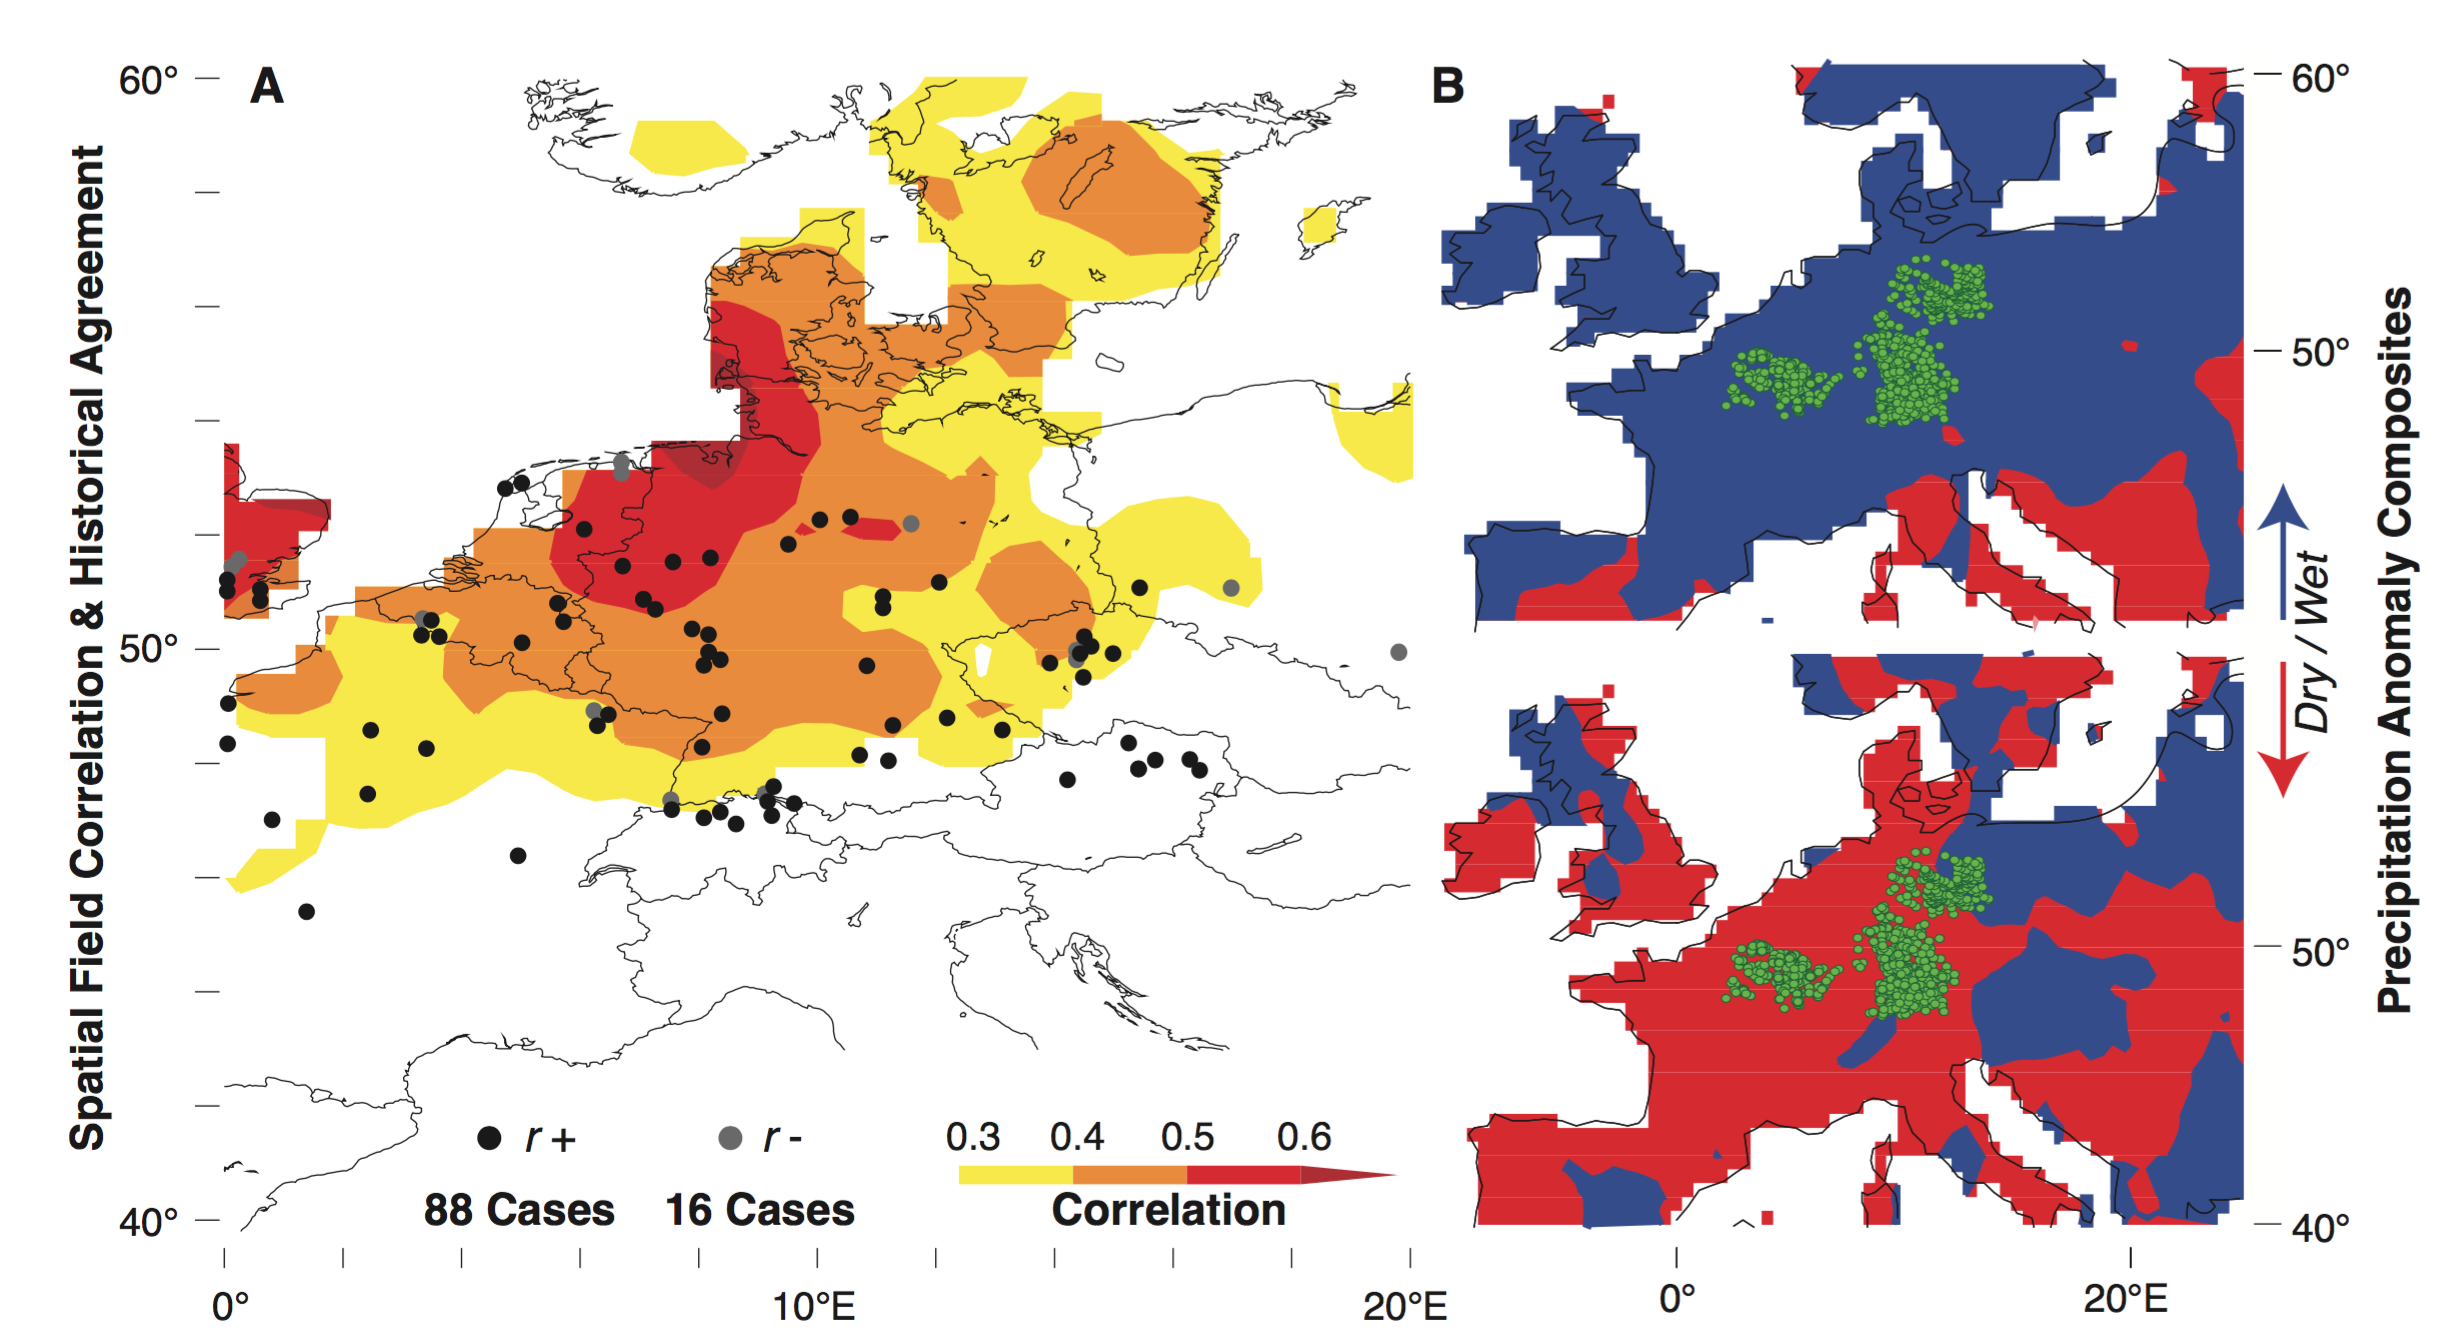
\includegraphics[width=1\textwidth]{BuntgenFig3}
	\begin{multicols}{2}
\caption{(\textbf{A}) Correlation map of the mean oak chronology against gridded central European AMJ precipitation data (1901–1980) together with the location of 104 historical reports, of which 88 witnesses corroborate 30 of 32 climatic extremes that were reconstructed from the oak data between 1013 and 1504, whereas 16 witnesses offer contradictory reports. Note that different reports may originate from the same location. (\textbf{B}) Composite anomaly fields (scaled means, modified t values) of summer (JJA) precipitation computed for 12 positive (top) and 16 negative (bottom) oak extremes between 1500 and 2000 (21). Significance of the composite anomalies, relative to the 1901–2000 climatology, was computed using 95\% confidence thresholds of the modified two-sided t test (21). Blue and red colors refer to significantly wet and dry conditions, respectively. Green dots refer to the location of 7284 central European oak samples.} 
	\end{multicols}	
\label{Fig3} 
\end{figure}

\begin{figure}[h]
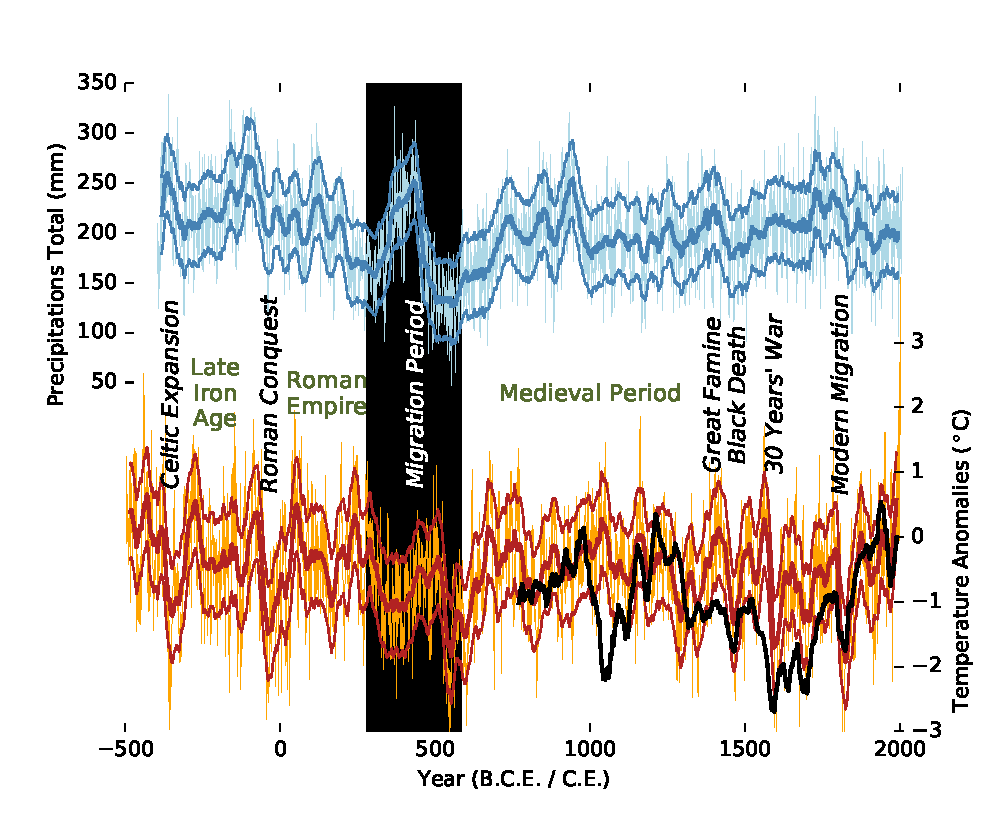
\includegraphics[width=1\textwidth]{BuntgenFig4_1}
	\begin{multicols}{2}
\caption{Reconstructed AMJ precipitation totals (\textbf{top}) and JJA temperature anomalies (\textbf{bottom}) with respect to the 1901–2000 period. Error bars are T1 RMSE of the calibration periods. Black lines show independent precipitation and temperature reconstructions from Germany (19) and Switzerland (18). Bold lines are 60-year low-pass filters. Periods of demographic expansion, economic prosperity, and societal stability are noted, as are periods of political turmoil, cultural change, and population instability.}
	\end{multicols}	
\label{Fig4}
\end{figure}
	\begin{multicols}{3}
The regional oak chronologies correlate on average at 0.39 with AMJ precipitation variability (1901–1980) averaged over 45 to 50N and 8 to 10E. Increased agreement between the tree-ring proxy and instrumental target records is obtained from the combined central European oak record, which correlates at 0.50 to 0.59 with interannual to multidecadal variations in AMJ precipitation (fig. S9). Correlation between this study and an independent summer drought reconstruction from central Germany (19) is 0.56 over the common 996 to 2005 C.E. period (Fig. \ref{Fig4}). To complement our hydroclimatic reconstruction,
we also developed a central European summer temperature proxy based on 1089 stone pine (\textit{Pinus cembra}) and 457 European larch (\textit{Larix decidua}) ring width series from high-elevation sites in the Austrian Alps and adjacent areas (21). This composite record includes living trees, historical timber, and subfossil wood, and correlates at 0.72 to 0.92 with interannual to multidecadal variations in instrumental June-to-August (JJA) temperature (1864–2003). The new proxy is significantly positive correlated with 20th century JJA temperatures of central Europe and the Mediterranean region (21), and possesses high- to low-frequency agreement with an independent maximum latewood density-based temperature surrogate from the Swiss Alps (18) (r = 0.35 to 0.44; 755 to 2003 C.E.) (Fig. \ref{Fig4}). \par
AMJ precipitation was generally above average and fluctuated within fairly narrow margins from the Late Iron Age through most of the Roman Period until ~250 C.E., whereas two depressions in JJA temperature coincided with the Celtic Expansion (~350 B.C.E.) and the Roman Conquest (~50 B.C.E.). Exceptional climate variability is reconstructed for ~250 to 550 C.E. and coincides with some of the most severe challenges in Europe’s political, social, and economic history, during the Migration Period. Distinct drying in the 3rd century paralleled a period of serious crisis in the WRE marked by barbarian invasion, political turmoil, and economic dislocation in several provinces of Gaul, including Belgica, Germania superior, and Rhaetia (24, 25). Precipitation increased during the recovery of the WRE in the 300s under the dynasties of Constantine and Valentinian, while temperatures were below average. Precipitation surpassed early
imperial levels during the demise of the WRE in the 5th century before dropping sharply in the first half of the 6th century. At the same time, falling
lake levels in Europe and Africa (1, 26) accompanied hemispheric-scale cooling that has been linked with an explosive near-equatorial volcanic eruption in 536 C.E. (27), followed by the first pandemic of Justinian plague that spread from the eastern Mediterranean in 542–543 C.E. (28). Rapid climate changes together with frequent epidemics had the overall capacity to disrupt the food production of agrarian societies (5–8).Most of the oak samples from this period originate from archaeological excavations of water wells and subfossil remains currently located in floodplains and wetlands (Fig. \ref{Fig2}D), possibly attesting to drier
conditions during their colonization. \par
AMJ precipitation and JJA temperature began to increase from the end of the 6th century C.E. and reached climate conditions comparable to those of the Roman period in the early 800s. The onset of wetter and warmer summers is contemporaneous with the societal consolidation of new kingdoms that developed in the
former WRE (23). Reduced climate variability from ~700 to 1000 C.E., relative to its surroundings, matches the new and sustained demographic growth in the northwest European countryside, and even the establishment of Norse colonies in the cold environments of Iceland and Greenland (9). Humid and mild summers paralleled the rapid cultural and political growth of medieval Europe under the Merovingian and Carolingian dynasties and their successors (23). Average precipitation and temperature showed fewer fluctuations during the period of peak medieval demographic and economic growth, ~1000 to 1200 C.E. (22, 23). Wetter summers during the 13th and 14th centuries and a first cold spell at ~1300 C.E. agree with the globally observed onset of the Little Ice Age (20, 29),
likely contributing to widespread famine across central Europe. Unfavorable climate may have even played a role in debilitating the underlying
health conditions that contributed to the devastating economic crisis that arose from the second plague pandemic, the BlackDeath, which reduced the central European population after 1347 C.E. by 40 to 60\% (19, 22, 28). The period is also associated with a temperature decline in the North Atlantic and the abrupt desertion of former Greenland settlements (9). Temperature minima in the early 17th and 19th centuries accompanied sustained settlement abandonment
during the Thirty Years’ War and the modern migrations from Europe to America. \par
The rate of natural precipitation and temperature change during the Migration Period may represent a natural analog to rates of projected
anthropogenic climate change. Although modern populations are potentially less vulnerable to climatic fluctuations than past societies
have been, they also are certainly not immune to the predicted temperature and precipitation changes, especially considering that migration
to more favorable habitats (22) as an adaptive response will not be an option in an increasingly crowded world (6). Comparison of climate
variability and human history, however, prohibits any simple causal determination; other contributing factors such as sociocultural stressors
must be considered in this complex interplay (7, 30). Nonetheless, the new climate evidence sets a paleoclimatic benchmark in terms of temporal
resolution, sample replication, and record length. \par
Our data provide independent evidence that agrarian wealth and overall economic growth might be related to climate change on high- to mid-frequency (interannual to decadal) time scales. Preindustrial societies were sensitive to famine, disease, and war, which were often driven by drought, flood, frost or fire events, as independently described by documentary archives (30). It also appears to be likely that societies can better compensate for abrupt (annual) climatic extremes and have the capacity to adapt to slower (multidecadal to centennial) environmental changes (6, 7). \par
The historical association of precipitation and temperature variation with population migration and settlement desertion in Europe may provide a basis for questioning the recent political and fiscal reluctance to mitigate projected global climate change (31), which reflects the common societal belief that civilizations are insulated from variations in the natural environment.

\section*{References and notes}
\bibliographystyle{plain} %conditionne l'affichage
\bibliography{BiblioBuntgenfinie}
%pour citer des refs dans le texte: 
%synchroniser sa base (dans le meme répertoire que le doc .tex) avec BibTex puis à l'endroit de la citation utiliser la commande \cite{référence dans  la base biblio}. puis synchroniser avec LaTeX avec BibTex et à nouveau avec LaTeX pour compiler le doc final.



32. We thank E. Cook, K. Gibson, G. Haug, G. Huang,
D. Johnson, M. Küttel, N. Stenseth, E. Zorita, and two
anonymous referees for comments and discussion.
Supported by the Swiss National Science Foundation
(NCCR-Climate), the Deutsche Forschungsgemeinschaft
projects PRIME (62201185) and Paleoclimatology of
the Middle East (62201236), the Austrian Science
Fund FWF (P15828, F3113-G02), l’Institut National
de Recherches Archéologiques Préventives, the
Andrew W. Mellon Foundation, and European Union
projects MILLENNIUM (017008), ACQWA (212250),
and CIRCE (036961).

\section*{\textbf{Supporting Online Material}}
www.sciencemag.org/cgi/content/ full/science.1197175/DC1 

Materials and Methods

Figs. S1 to S12

Tables S1 and S2

References

31 August 2010; accepted 5 January 2011 Published online 13 January 2011; 10.1126/science.1197175
	
	
	
	
	
	
	
	
\end{multicols}	
\end{myfont}	
\end{document}